\chapter{Modell}
%\section{Hameltonien}
Um den Inversen Farady-Effekt mit Hilfe der Floquet-Theorie in
einem Bandisolator genauer zu untersuchen soll hier ein einfaches 2D-Modell
eines Festkörpers mit vier Positionen herangezogen werden.
Die Postionen sind im Abstand der Gitterkonstante $d$ quadratisch angeordnet.
Der Bandisolator wird durch
genau wechselnde lokale Energien $a$ dargestellt.
In dem System soll sich zunächst nur ein Elektron befinden, welches mit der Energie
$J$ zu den nächsten Nachbarn hüfen kann.
In der Abbildung \ref{fig:sytem}
ist das zu untersuchende System noch einmal bildlich dargestellt.

\begin{figure}
   \centering
   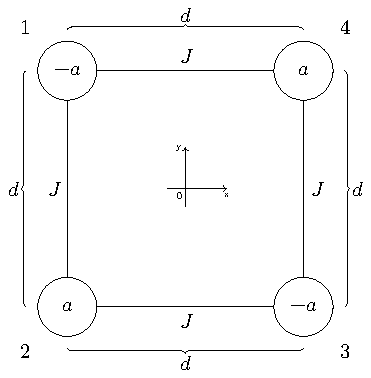
\includegraphics[width=0.5\textwidth]{C:/Users/daghe/Desktop/Uni/Bachelorarbeit/Tikz_test/bild_gitter_0.pdf}
   \caption{System.}
   \label{fig:system}
\end{figure}

\section{Zeitunabhängiges System}
Solch ein System lässt sich durch
ein Tight-Binding-Modell in zweiter Quantisierung beschreiben.
Aus dem Tight-Binding-Modell ergibt sich der folgende Hamiltonian $H_0$ für das zeitunabhängige Systems % lautet
\begin{align}
  H_0=J\sum_{i=1}^4 \left(c_{i+1}^\dag c_i^{\phantom{\dag}} + c_{i}^\dag c_{i+1}^{\phantom{\dag}}   +a_i^{\phantom{\dag}} c_i^\dag c_i^{\phantom{\dag}}\right).
\end{align}
Durch die Wahl einer Basis, hier
\begin{align}
 \ket{1}=\vec{e_1}&  &\ket{2}=\vec{e_2}&  &\ket{2}=\vec{e_2}& &\ket{3}=\vec{e_3}& &\ket{4}=\vec{e_4},
\intertext{kann über}
H_{ji}=\braket{j|H|i}
\intertext{die Matrixdarstellung des Hamiltonian}
  H_0=\begin{pmatrix}
  -a& \phantom{-}J& & \phantom{-}J \\
  \phantom{-}J& a &\phantom{-}J & 0\\
  0& \phantom{-}J& -a& \phantom{-}J \\
  \phantom{-}J& 0&  \phantom{-}J & \phantom{-}a
\end{pmatrix}
\end{align}
bestimmt werden.
Durch die stationäre Schrödinger Gleichung
können nun die Eigenwerte $E_i$ und Eigenvektoren $\ket{\phi_i}$  des Hamiltonian bestimmt werden.
Die Eigenwerte des zeitunabhängigen Systems sind:
\begin{align}
  E_{1/4}&=\mp\sqrt{a^2+4J^2}&  &E_{2/3}=\mp a
\end{align}
So ergibt sich das in der Abbildung \ref{fig:bandstrucktur} dargestellte Niveauschema.
\begin{figure}
   \centering
   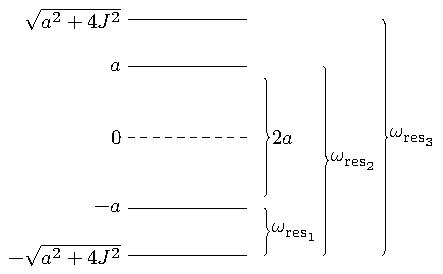
\includegraphics[width=0.4\textwidth]{C:/Users/daghe/Desktop/Uni/Bachelorarbeit/Tikz_test/bild_niveau.pdf}
   \caption{Niveauschema für ein Elektron im System.}
   \label{fig:bandstrucktur}
\end{figure}

%Ebenfalls kann die für ein Bandisolator charakteristische Bandlücke von $2a$
Aus dem Niveauschema können die Resonanzfrequenzen des Systems im Grundzustand entnommen werden.
\begin{align}
\omega_{\text{res}_1}=\sqrt{a^2+4J^2}-a
& &\omega_{\text{res}_2}=a+\sqrt{a^2+4J^2}
& &\omega_{\text{res}_3}=2\sqrt{a^2+4J^2}
\end{align}

\section{Zeitabhängiges System}
Nun soll das System durch ein sich in der Mitte befindendes rotierendes E-Feld erweitert werden, welches
das zirkular polarisierte Licht simulieren soll (Abbildung:\ref{fig:syst+E}).

\begin{figure}
   \centering
   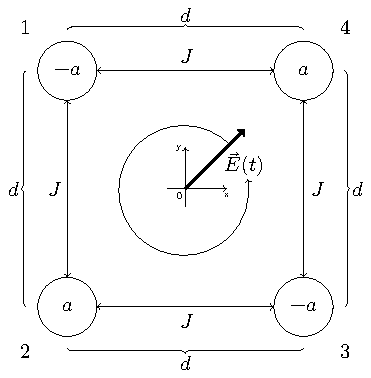
\includegraphics[width=0.4\textwidth]{C:/Users/daghe/Desktop/Uni/Bachelorarbeit/Tikz_test/bild_gitter.pdf}
   \caption{System+E-Feld.}
   \label{fig:syst+E}
\end{figure}


Der Hamiltonian wird dafür um den Term
\begin{align}
  \sum_{i=1}^4 \epsilon_i^{\phantom{\dag}} c_i^\dag c_i^{\phantom{\dag}}  \,\,   \text{mit} \,\, \epsilon=-\vec{E} \vec{r_i}
\end{align}
erweitert. Dabei beschreibt $\vec E$ das E-Feld
\begin{align}
  \vec E=E_0\begin{pmatrix}
\cos\left(\omega t+\upphi\right)\\
\sin\left(\omega t+\upphi\right)
 \end{pmatrix},
 \intertext{welches die Amplitude $E_0$ ,die Frequenz $\omega$ und die Phase $\upphi$ besitzt}
\end{align}
Der Ursprung des Systems wird einfachshalber in dem Mittelpunkt des Systems gesetzt
somit lässt sich $r_i$, der Vektor welcher (ADD) Position zeigt, in Abhänigigkeit von der Gitterkonstante $d$ schreiben.
\begin{align}
  r_1=\frac{1}{2}\begin{pmatrix}-d  \\ \phantom{-}d \end{pmatrix}& &
  r_2=\frac{1}{2}\begin{pmatrix}-d  \\ -d \end{pmatrix}& &
  r_3=\frac{1}{2}\begin{pmatrix}\phantom{-}d  \\ -d \end{pmatrix}& &
  r_4=\frac{1}{2}\begin{pmatrix}d  \\ d \end{pmatrix}
\end{align}
Der gesamte Hamiltonian des Systems nimmt somit die Form
\begin{align}
H=J\sum_{i=1}^4 \left(c_{i+1}^\dag c_i^{\phantom{\dag}} + c_{i}^\dag c_{i+1}^{\phantom{\dag}}   +a_i^{\phantom{\dag}} c_i^\dag c_i^{\phantom{\dag}} +\epsilon_i^{\phantom{\dag}} c_i^\dag c_i^{\phantom{\dag}}\right)\\
H=J\sum_{i=1}^4 \left(c_{i+1}^\dag c_i^{\phantom{\dag}} + c_{i}^\dag c_{i+1}^{\phantom{\dag}}   +a_i^{\phantom{\dag}} c_i^\dag c_i^{\phantom{\dag}} -\vec{E} \vec{r_i}  c_i^\dag c_i^{\phantom{\dag}}\right)\\
\end{align}
an.


\section{Floquetmatrix des gestörten Systems}
Für das Zeitabhängige System soll nun wie in Kapitel \ref{sec:numerisch} beschrieben die numerische Methode der Floquet-Matrix angewendet werden.
Dafür kann zunächst der Hamiltonien
\begin{align}
H=\underbrace{J\sum_{i=1}^4 \left(c_{i+1}^\dag c_i^{\phantom{\dag}} + c_{i}^\dag c_{i+1}^{\phantom{\dag}}c_i^{\phantom{\dag}} + a_i^{\phantom{\dag}} c_i^\dag c_i^{\phantom{\dag}}
 \right)}_{H_0} +\underbrace{\sum_{i=1}^4\left(\epsilon_i^{\phantom{\dag}} c_i^\dag c_i^{\phantom{\dag}}\right)}_{V(t)}
\end{align}
in den zuvor behandelten zeitunabhänigen Teil $H_0$ und einen in der Zeit periodischen Teil $V(t)$ aufgespalten werden.
Um die Matrix $\mathcal{H}_\mathrm{F}$ zu berechnenen, werden zunächst die Untermatrizen $H^{m-n}$
durch die Gleichung \eqref{eqn:H_n_m} berechnet.
Das Ergebniss lautet
\begin{align}
  H^{m-n}=H_0\delta_{m,n} -\frac{E_0}{2}\left(R_{(-)} \exp\left( \mathrm{i}\upphi\right)\delta_{n+1,m}   +  R_{(+)}\exp\left( -\mathrm{i}\upphi\right)\delta_{n-1,m}\right)\\
\end{align}
mit
\begin{align}
  R_{(-)}=
\begin{pmatrix}
  r_{1_x}-r_{1_y}& & & \\
  &r_{2_x}-r_{2_y} & & \\
  & & r_{3_x}-r_{3_y}& \\
  & & & r_{4_x}-r_{4_y}
\end{pmatrix}\\
R_{(+)}= \text{diag}\left(
r_{1_x}+r_{1_y},
r_{2_x}+r_{2_y},
r_{3_x}+r_{3_y},
r_{4_x}+r_{4_y}\right).
\end{align}
Somit ergibt sich für die Martix $\mathcal{H}_F$ nach der Gleichung \eqref{eqn:H_f} in
Blockschreibweise zu einer Diagonalbandmatix.
\begin{align}
  \mathcal{H}_F=\begin{pmatrix}
  H^{-n ,-n}+(-n)\hbar\omega  &  H^{-n,-n+1}       &       &    & \\
  H^{-n+1,-n} &    H^{-n+1,-n+1}+(1-n)\hbar\omega  & \ddots&    & \\
            &          \ddots                      & \ddots&  \ddots      &    \\
            &                                      & \ddots&  H^{n-1,n-1}+(n-1)\hbar\omega  & H^{n-1,n}  \\
            &                                      &       & H^{n,n-1}   & H^{n,n}
\end{pmatrix}
\end{align}
Um die die genauen $\epsilon_{\alpha}$ und $\ket{\Phi_\alpha}$ zu berechen, ist es Notwendig das $n\rightarrow\infty $.
Dies ist numerisch jedoch nicht möglich, folglich muss die Matrix bei einem beliebigen $n$ trunkiert werden.
Die Matrix $\mathcal{H}_F$ für eine Trukierung bei $n=1$ würde beispielsweise diese Form
\begin{align}
  \mathcal{H}_F=\begin{pmatrix}
  H^{-1,-1}-\mathbb{1}\hbar\omega &  H^{-1,0} &   0 \\
  H^{0,-1}               &  H^{0,0}  &H^{0,1}                  \\
      0                  &  H^{1,0}  & H^{1,1}+\mathbb{1}\hbar\omega
\end{pmatrix}
\end{align}
besitzen.

\section{Abschätzen der Größenordnungen}
